% 图 51.2 —— 由 `checks/emit_hand.py` 自动拼出（probe 精测 + prims2 图元分解）
%%
% ⚠ 这是**稿子不是成品**：跑 `checks/checkhand.py 51.2` 看指标 + 看叠合图。
%%
%% ⚠ 待核：
%   · 本图 probe 报出阴影族 3 个 —— **本脚本不生成阴影**（要照原书手写）；prims2 的 strokes 里可能含阴影线，核对时留意别画重
%   · 可疑字形 1 项（空心圈 ⊙ 常被认成字母 o）—— 见文件末
%%
\documentclass[12pt]{standalone}
\usepackage{fontspec}
\setsansfont{Arial}
\newfontfamily\mfallback{DejaVu Sans}
\usepackage{tikz}
\usetikzlibrary{arrows.meta}
\begin{document}
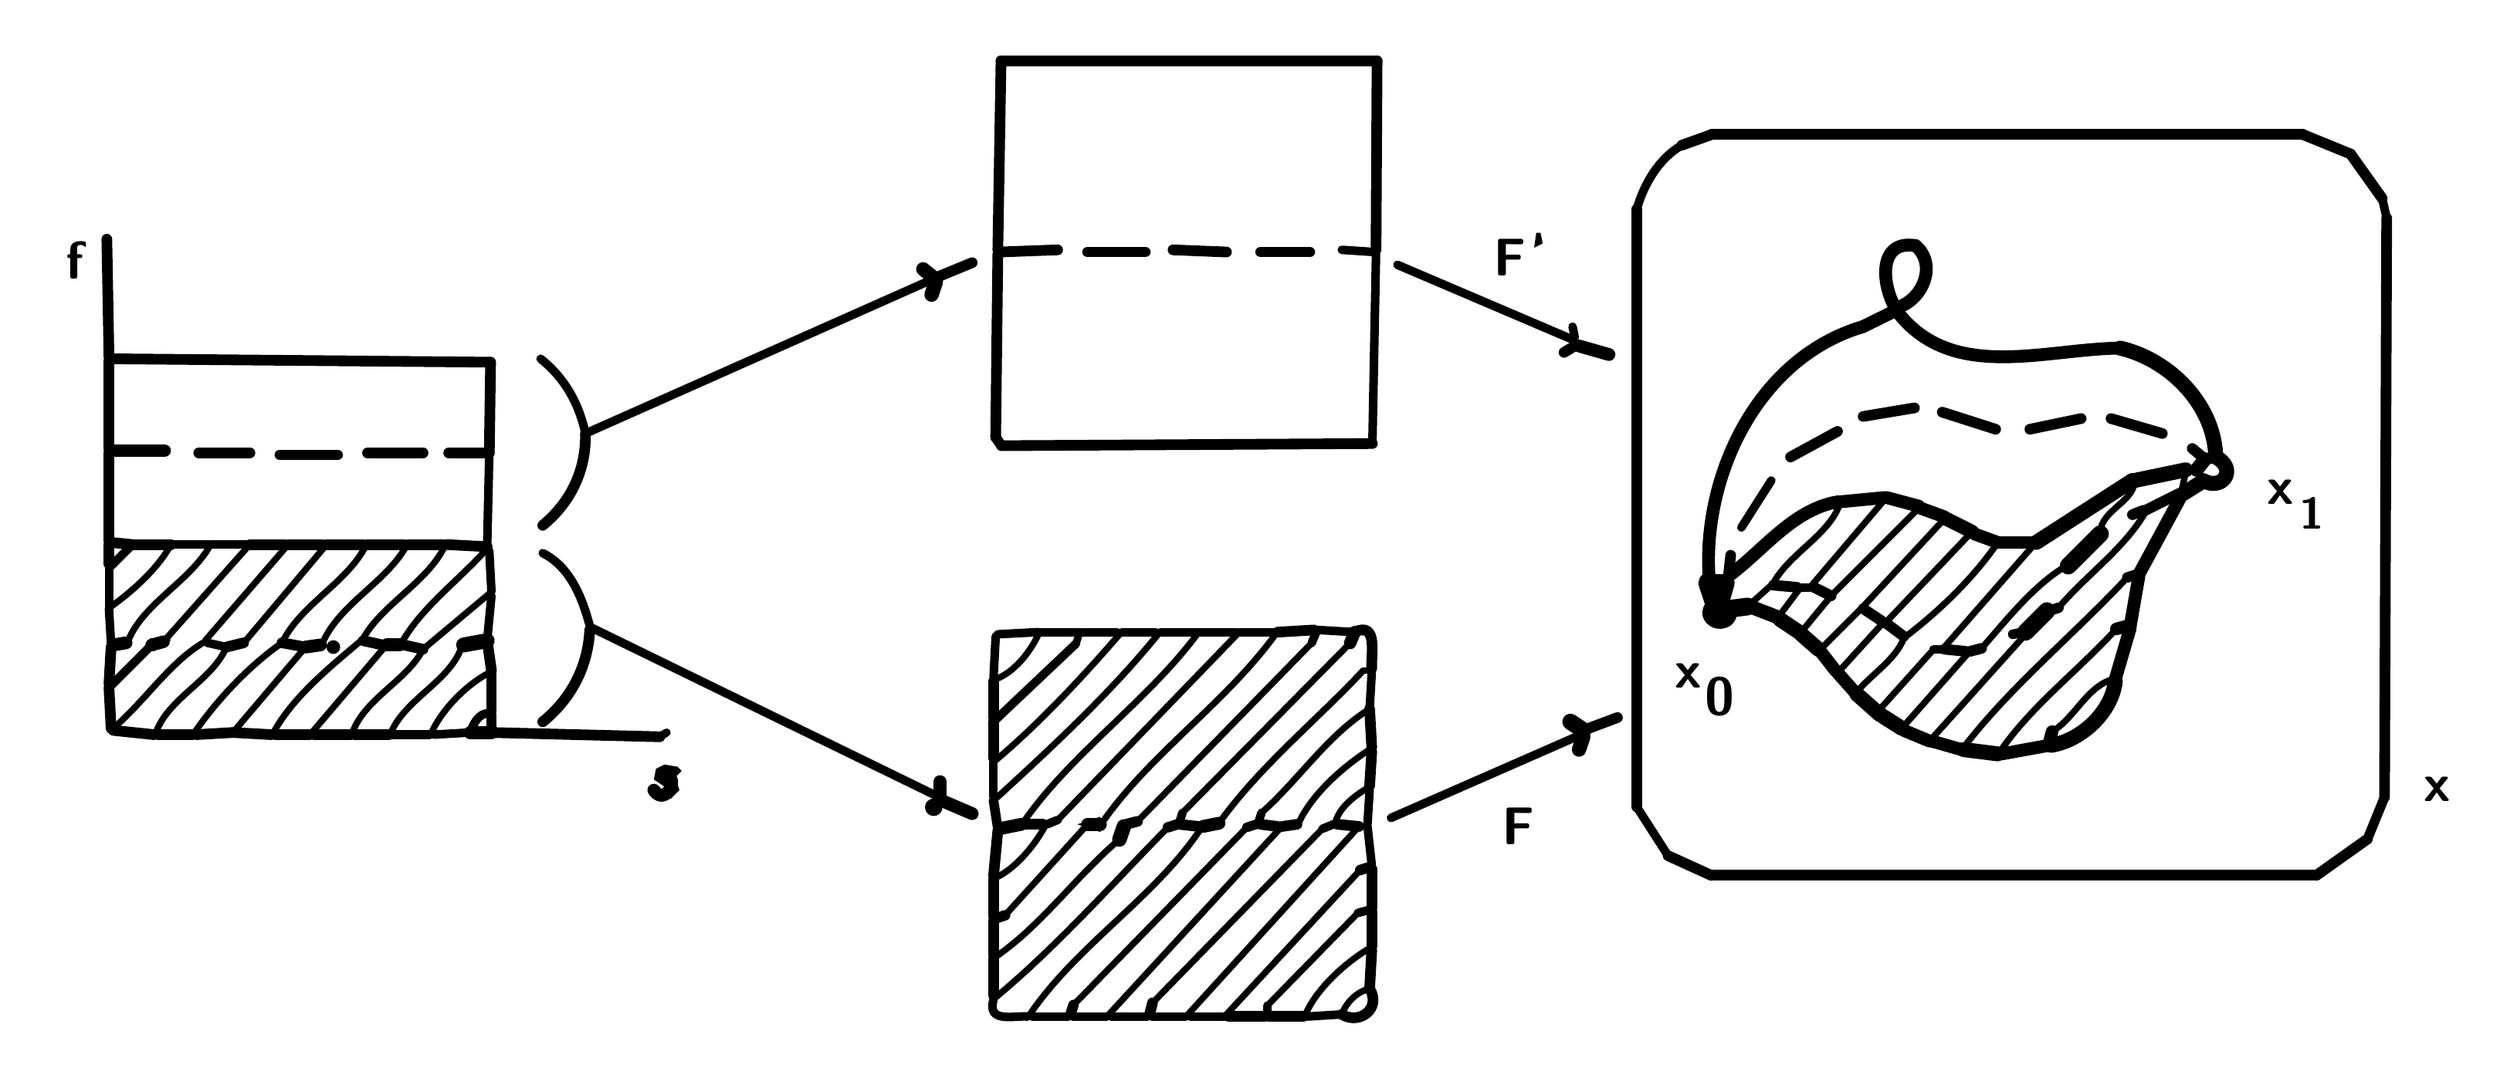
\begin{tikzpicture}[x=1pt, y=-1pt, line width=6.0pt, line cap=round, line join=round]

  %% ════ 填充区（prims2 的 fills）════
  \fill (307.0,349.0) -- (301.0,348.0) -- (297.0,350.0) -- (296.0,355.0) -- (302.0,359.0) -- (300.0,361.0) -- (295.0,359.0) -- (296.0,363.0) -- (304.0,364.0) -- (308.0,360.0) -- (306.0,354.0) -- (309.0,351.0) -- cycle;
  \fill (711.0,99.0) -- (709.0,99.0) -- (708.0,106.0) -- (712.0,104.0) -- cycle;

  %% ════ 直线段（prims2 的 strokes）════
  \draw[line width=6.0pt] (177.0,292.0) -- (171.0,292.0);
  \draw[line width=4.0pt] (641.0,373.0) -- (730.0,334.0);
  \draw[line width=4.0pt] (632.0,305.0) -- (631.0,322.0);
  \draw[line width=5.0pt] (603.0,108.0) -- (580.0,108.0);
  \draw[line width=3.0pt] (629.0,377.0) -- (626.0,377.0);
  \draw[line width=5.0pt] (42.0,158.0) -- (219.6,159.6);
  \draw[line width=5.0pt] (219.6,159.6) -- (219.0,202.0);
  \draw[line width=4.0pt] (833.0,265.0) -- (837.0,265.0);
  \draw[line width=4.0pt] (42.0,292.0) -- (41.0,275.0);
  \draw[line width=5.0pt] (634.0,107.0) -- (634.5,18.5);
  \draw[line width=5.0pt] (634.5,18.5) -- (458.5,18.5);
  \draw[line width=5.0pt] (458.5,18.5) -- (457.0,107.0);
  \draw[line width=4.9pt] (456.0,420.0) -- (460.4,418.6);
  \draw[line width=3.0pt] (460.4,418.6) -- (499.0,376.0);
  \draw[line width=6.0pt] (499.0,376.0) -- (505.0,376.0);
  \fill (505.0,372.4) -- (505.0,379.6) -- (494.2,376.0) -- cycle;
  \draw[line width=6.0pt] (791.0,262.0) -- (797.0,262.0);
  \draw[line width=4.0pt] (457.0,287.0) -- (476.0,286.0);
  \draw[line width=4.0pt] (579.0,375.0) -- (580.4,370.6);
  \draw[line width=7.0pt] (869.0,324.0) -- (880.0,331.0);
  \draw[line width=6.5pt] (422.0,116.0) -- (427.0,120.0);
  \draw[line width=3.0pt] (631.0,304.0) -- (628.0,304.0);
  \draw[line width=6.0pt] (560.5,375.5) -- (553.0,377.0);
  \draw[line width=5.0pt] (107.0,202.0) -- (83.0,202.0);
  % （略）线段 (507.0,376.0)-(515.0,376.0) 线宽6.0 —— 是箭头头那一坨，已由箭头头代替
  \draw[line width=3.0pt] (569.0,287.0) -- (485.1,373.9);
  \draw[line width=4.0pt] (485.1,373.9) -- (480.0,376.0);
  \draw[line width=6.0pt] (458.0,378.0) -- (468.0,376.0);
  \draw[line width=5.0pt] (632.0,433.0) -- (632.0,417.0);
  \draw[line width=5.0pt] (455.0,400.0) -- (457.0,379.0);
  \draw[line width=6.0pt] (430.0,356.0) -- (430.0,362.0);
  \draw[line width=3.0pt] (136.0,333.0) -- (170.0,293.0);
  \draw[line width=5.0pt] (428.0,120.0) -- (445.0,113.0);
  \draw[line width=5.0pt] (119.0,334.0) -- (135.0,334.0);
  \draw[line width=5.0pt] (181.0,245.0) -- (197.0,245.0);
  \draw[line width=5.0pt] (219.0,202.0) -- (200.0,202.0);
  \draw[line width=4.0pt] (219.0,202.0) -- (218.0,246.0);
  \draw[line width=5.0pt] (137.0,334.0) -- (154.0,334.0);
  \draw[line width=5.0pt] (199.0,245.0) -- (218.0,246.0);
  \draw[line width=5.0pt] (485.0,107.0) -- (458.0,108.0);
  \draw[line width=4.0pt] (632.0,395.0) -- (630.0,377.0);
  \draw[line width=6.0pt] (140.0,292.0) -- (133.0,293.0);
  \draw[line width=6.0pt] (908.0,341.0) -- (894.0,337.0);
  \draw[line width=4.0pt] (429.0,363.0) -- (267.0,284.0);
  \draw[line width=5.0pt] (1010.0,221.0) -- (994.0,229.0);
  \draw[line width=4.0pt] (264.0,193.0) -- (426.0,121.0);
  \draw[line width=3.0pt] (809.0,273.0) -- (819.0,264.0);
  \draw[line width=7.0pt] (841.0,294.0) -- (833.0,287.0);
  \draw[line width=6.0pt] (49.0,291.0) -- (43.0,292.0);
  \draw[line width=4.0pt] (542.0,375.0) -- (543.4,370.6);
  \draw[line width=3.0pt] (543.4,370.6) -- (621.9,291.1);
  \draw[line width=5.8pt] (621.9,291.1) -- (624.0,286.0);
  \draw[line width=4.0pt] (614.0,376.0) -- (608.9,378.1);
  \draw[line width=3.0pt] (608.9,378.1) -- (529.4,459.6);
  \draw[line width=5.0pt] (529.4,459.6) -- (528.0,465.0);
  \draw[line width=4.5pt] (932.0,287.0) -- (937.0,286.0);
  \draw[line width=4.0pt] (41.0,256.0) -- (41.0,274.0);
  \draw[line width=5.0pt] (41.0,245.0) -- (41.0,254.0);
  \draw[line width=5.0pt] (470.0,376.0) -- (478.0,376.0);
  \draw[line width=3.0pt] (871.0,282.0) -- (851.0,304.0);
  \draw[line width=7.0pt] (832.0,286.0) -- (823.0,280.0);
  \draw[line width=4.0pt] (607.0,285.0) -- (624.0,286.0);
  \draw[line width=6.0pt] (991.0,259.0) -- (1011.0,222.0);
  \draw[line width=4.0pt] (583.0,465.0) -- (583.0,461.0);
  \draw[line width=3.0pt] (583.0,461.0) -- (625.5,417.5);
  \draw[line width=4.0pt] (625.5,417.5) -- (631.0,416.0);
  \draw[line width=7.0pt] (1020.0,216.0) -- (1012.0,221.0);
  \draw[line width=5.0pt] (162.0,245.0) -- (179.0,245.0);
  \draw[line width=6.0pt] (850.0,305.0) -- (858.0,314.0);
  \draw[line width=4.0pt] (529.0,466.0) -- (545.0,466.0);
  \draw[line width=6.0pt] (729.0,152.0) -- (743.0,156.0);
  \draw[line width=3.0pt] (862.0,274.0) -- (900.0,233.0);
  \draw[line width=4.5pt] (455.0,365.0) -- (457.0,378.0);
  \draw[line width=5.0pt] (220.0,323.0) -- (220.0,306.0);
  \draw[line width=5.0pt] (912.0,295.0) -- (917.4,293.6);
  \draw[line width=5.0pt] (747.0,326.0) -- (731.0,332.0);
  \draw[line width=5.0pt] (940.0,191.0) -- (964.0,186.0);
  \draw[line width=4.9pt] (949.0,276.0) -- (953.4,274.6);
  \draw[line width=6.0pt] (849.0,304.0) -- (842.0,295.0);
  \draw[line width=3.0pt] (546.0,465.0) -- (626.0,377.0);
  \draw[line width=5.3pt] (1027.0,204.0) -- (1022.0,205.0);
  \draw[line width=5.0pt] (220.0,304.0) -- (218.0,290.0);
  \draw[line width=5.0pt] (143.0,245.0) -- (160.0,245.0);
  \draw[line width=3.0pt] (564.0,465.0) -- (626.6,397.4);
  \draw[line width=4.9pt] (626.6,397.4) -- (631.0,396.0);
  \draw[line width=4.9pt] (990.0,259.0) -- (985.6,260.4);
  \draw[line width=3.0pt] (823.0,278.0) -- (832.0,266.0);
  \draw[line width=4.0pt] (492.0,466.0) -- (508.0,466.0);
  \draw[line width=4.0pt] (193.0,334.0) -- (210.0,333.0);
  \draw[line width=7.0pt] (925.0,343.0) -- (909.0,341.0);
  \draw[line width=4.0pt] (510.0,466.0) -- (527.0,466.0);
  \draw[line width=4.0pt] (570.0,286.0) -- (587.0,286.0);
  \draw[line width=5.0pt] (881.0,288.0) -- (873.0,282.0);
  \draw[line width=6.0pt] (873.0,223.0) -- (888.0,227.0);
  \draw[line width=4.0pt] (631.0,360.0) -- (630.0,376.0);
  \draw[line width=6.0pt] (987.0,284.0) -- (980.0,308.0);
  \draw[line width=8.0pt] (938.0,286.0) -- (948.0,276.0);
  \draw[line width=6.0pt] (941.0,244.0) -- (925.0,244.0);
  \draw[line width=4.0pt] (220.0,269.0) -- (218.0,290.0);
  \draw[line width=5.0pt] (41.0,202.0) -- (41.0,243.0);
  \draw[line width=5.0pt] (42.0,331.0) -- (41.0,312.0);
  \draw[line width=6.0pt] (949.0,339.0) -- (927.0,343.0);
  \draw[line width=3.0pt] (942.0,245.0) -- (900.0,293.0);
  \draw[line width=6.0pt] (431.0,365.0) -- (445.0,371.0);
  \draw[line width=5.0pt] (62.0,334.0) -- (43.0,332.0);
  \draw[line width=5.0pt] (162.0,202.0) -- (188.0,202.0);
  \draw[line width=5.0pt] (42.0,293.0) -- (41.0,310.0);
  \draw[line width=5.0pt] (80.0,334.0) -- (64.0,334.0);
  \draw[line width=5.0pt] (580.0,376.0) -- (588.0,377.0);
  \draw[line width=4.0pt] (473.0,466.0) -- (490.0,466.0);
  \draw[line width=4.0pt] (515.0,286.0) -- (531.0,286.0);
  \draw[line width=4.0pt] (174.0,334.0) -- (191.0,334.0);
  \draw[line width=5.0pt] (42.0,244.0) -- (52.0,245.0);
  \draw[line width=4.0pt] (533.0,286.0) -- (551.0,286.0);
  \draw[line width=3.0pt] (219.0,268.0) -- (188.0,294.0);
  \draw[line width=4.0pt] (551.0,286.0) -- (569.0,286.0);
  \draw[line width=5.0pt] (455.0,456.0) -- (455.0,439.0);
  % （略）线段 (60.0,292.0)-(51.0,291.0) 线宽4.0 —— 是箭头头那一坨，已由箭头头代替
  \draw[line width=5.0pt] (104.0,291.0) -- (96.0,293.0);
  \draw[line width=5.0pt] (1002.0,193.0) -- (978.0,186.0);
  \draw[line width=6.0pt] (872.0,223.0) -- (851.0,225.0);
  \draw[line width=6.0pt] (67.0,201.0) -- (42.0,201.0);
  \draw[line width=6.5pt] (1018.0,210.0) -- (1022.0,205.0);
  \draw[line width=4.2pt] (796.0,271.0) -- (799.0,274.0);
  \draw[line width=5.0pt] (988.0,231.0) -- (993.0,229.0);
  \draw[line width=6.7pt] (729.0,341.0) -- (731.0,335.0);
  \draw[line width=5.0pt] (121.0,203.0) -- (148.0,203.0);
  \draw[line width=7.0pt] (989.0,215.0) -- (1013.0,210.0);
  \draw[line width=5.0pt] (455.0,437.0) -- (455.0,421.0);
  \draw[line width=5.0pt] (123.0,245.0) -- (107.0,245.0);
  \draw[line width=5.0pt] (900.0,294.0) -- (910.0,295.0);
  \draw[line width=5.0pt] (924.0,191.0) -- (899.0,183.0);
  \draw[line width=5.0pt] (799.0,259.0) -- (800.0,250.0);
  \draw[line width=5.0pt] (499.0,108.0) -- (526.0,108.0);
  \draw[line width=6.8pt] (516.0,377.0) -- (513.9,383.1);
  \draw[line width=4.0pt] (496.0,286.0) -- (513.0,286.0);
  \draw[line width=5.0pt] (539.0,107.0) -- (564.0,108.0);
  \draw[line width=3.8pt] (302.0,333.0) -- (298.8,335.0);
  \draw[line width=5.0pt] (298.8,335.0) -- (220.0,333.0);
  \draw[line width=5.0pt] (584.0,466.0) -- (600.0,466.0);
  \draw[line width=4.0pt] (726.0,143.0) -- (727.0,148.0);
  \draw[line width=4.0pt] (602.0,466.0) -- (618.0,465.0);
  \draw[line width=4.0pt] (895.0,294.0) -- (899.0,294.0);
  \draw[line width=3.0pt] (895.0,294.0) -- (869.0,323.0);
  \draw[line width=6.0pt] (991.0,260.0) -- (987.0,283.0);
  \draw[line width=6.0pt] (861.8,143.0) -- (876.0,136.0);
  \draw[line width=3.0pt] (1017.0,210.0) -- (1014.0,210.0);
  \draw[line width=5.0pt] (632.0,415.0) -- (632.0,397.0);
  \draw[line width=5.0pt] (862.0,185.0) -- (886.0,181.0);
  \draw[line width=6.0pt] (881.0,332.0) -- (893.0,337.0);
  \draw[line width=7.0pt] (988.0,215.0) -- (943.0,244.0);
  \draw[line width=5.0pt] (542.0,376.0) -- (551.0,377.0);
  \draw[line width=4.0pt] (477.0,286.0) -- (495.0,286.0);
  \draw[line width=5.0pt] (172.0,334.0) -- (156.0,334.0);
  \draw[line width=4.0pt] (455.0,363.0) -- (455.0,347.0);
  \draw[line width=4.0pt] (547.0,466.0) -- (563.0,466.0);
  \draw[line width=4.0pt] (644.0,114.0) -- (726.0,149.0);
  \draw[line width=5.9pt] (980.5,284.5) -- (986.0,283.0);
  \draw[line width=5.0pt] (565.0,466.0) -- (582.0,466.0);
  \draw[line width=6.5pt] (913.0,239.0) -- (901.0,233.0);
  \draw[line width=5.0pt] (831.0,265.0) -- (820.0,264.0);
  \draw[line width=6.7pt] (426.0,128.0) -- (428.0,122.0);
  \draw[line width=6.0pt] (914.0,240.0) -- (925.0,244.0);
  \draw[line width=5.0pt] (631.0,453.0) -- (632.0,435.0);
  \draw[line width=5.0pt] (41.0,159.0) -- (41.0,200.0);
  \draw[line width=3.7pt] (794.0,273.0) -- (793.0,274.0);
  \draw[line width=7.0pt] (218.0,290.0) -- (207.0,292.0);
  \draw[line width=5.0pt] (188.0,294.0) -- (179.0,292.0);
  \draw[line width=4.0pt] (618.0,107.0) -- (633.0,108.0);
  \draw[line width=5.0pt] (117.0,334.0) -- (99.0,333.0);
  \draw[line width=3.0pt] (873.0,281.0) -- (912.0,240.0);
  \draw[line width=7.6pt] (725.0,328.0) -- (731.0,332.0);
  \draw[line width=5.0pt] (590.0,377.0) -- (597.0,376.0);
  \draw[line width=5.0pt] (588.0,286.0) -- (605.0,285.0);
  \draw[line width=4.0pt] (606.0,286.0) -- (603.9,291.1);
  \draw[line width=3.0pt] (603.9,291.1) -- (522.4,374.6);
  \draw[line width=5.0pt] (522.4,374.6) -- (517.0,376.0);
  \draw[line width=5.0pt] (626.0,377.0) -- (616.0,376.0);
  \draw[line width=5.0pt] (631.0,358.0) -- (632.0,342.0);
  \draw[line width=5.0pt] (862.0,275.0) -- (871.0,281.0);
  \draw[line width=6.0pt] (900.0,232.0) -- (889.0,228.0);
  \draw[line width=10.2pt] (793.0,272.0) -- (790.0,263.0);
  \draw[line width=4.0pt] (220.0,267.0) -- (219.0,248.0);
  \draw[line width=3.0pt] (1011.0,220.0) -- (1013.0,211.0);
  \draw[line width=5.0pt] (455.0,328.0) -- (455.0,345.0);
  \draw[line width=4.9pt] (536.6,377.4) -- (541.0,376.0);
  \draw[line width=5.0pt] (1022.0,205.0) -- (1016.0,200.0);
  \draw[line width=4.0pt] (60.0,293.0) -- (42.0,311.0);
  \draw[line width=3.0pt] (838.0,264.0) -- (872.0,224.0);
  \draw[line width=5.0pt] (455.0,309.0) -- (455.0,326.0);
  \draw[line width=3.0pt] (106.0,246.0) -- (66.5,290.5);
  \draw[line width=5.9pt] (66.5,290.5) -- (61.0,292.0);
  \fill (61.8,295.1) -- (60.2,288.9) -- (70.3,289.5) -- cycle;
  \draw[line width=5.0pt] (52.0,245.0) -- (70.0,245.0);
  \draw[line width=4.0pt] (52.0,245.0) -- (42.0,255.0);
  \draw[line width=5.0pt] (727.0,152.0) -- (722.0,155.0);
  \draw[line width=3.0pt] (124.0,246.0) -- (86.0,290.0);
  \draw[line width=3.0pt] (142.0,246.0) -- (105.0,290.0);
  \draw[line width=5.0pt] (122.0,291.0) -- (133.0,293.0);
  \draw[line width=6.5pt] (822.0,279.0) -- (809.0,274.0);
  \draw[line width=5.0pt] (631.0,322.0) -- (632.0,340.0);
  \draw[line width=3.0pt] (938.0,287.0) -- (894.0,336.0);
  \draw[line width=5.9pt] (950.4,332.6) -- (949.0,338.0);
  \draw[line width=3.0pt] (888.0,228.0) -- (847.0,269.0);
  \draw[line width=3.0pt] (842.0,294.0) -- (861.0,275.0);
  \draw[line width=5.0pt] (455.0,419.0) -- (455.0,402.0);
  \draw[line width=5.0pt] (141.0,245.0) -- (125.0,245.0);
  \draw[line width=3.0pt] (833.0,286.0) -- (847.0,269.0);
  \draw[line width=5.0pt] (41.0,157.0) -- (40.0,102.0);
  \draw[line width=5.0pt] (847.0,269.0) -- (839.0,265.0);
  \draw[line width=8.0pt] (958.0,255.0) -- (973.0,240.0);
  \draw[line width=3.0pt] (881.0,330.0) -- (911.0,296.0);
  \draw[line width=7.0pt] (868.0,323.0) -- (859.0,315.0);
  \draw[line width=4.0pt] (634.0,109.0) -- (632.3,197.7);
  \draw[line width=5.0pt] (632.3,197.7) -- (458.7,198.7);
  \draw[line width=4.8pt] (458.7,198.7) -- (456.0,194.8);
  \draw[line width=5.0pt] (456.0,194.8) -- (457.0,109.0);
  \draw[line width=4.0pt] (456.0,288.0) -- (455.0,307.0);
  \draw[line width=4.5pt] (578.0,376.0) -- (573.6,377.4);
  \draw[line width=3.0pt] (573.6,377.4) -- (492.4,460.6);
  \draw[line width=4.9pt] (492.4,460.6) -- (491.0,465.0);
  \draw[line width=4.0pt] (456.0,327.0) -- (493.6,291.4);
  \draw[line width=3.5pt] (493.6,291.4) -- (495.0,287.0);
  \draw[line width=3.0pt] (99.0,333.0) -- (133.0,293.0);
  \draw[line width=5.0pt] (99.0,333.0) -- (82.0,334.0);
  \draw[line width=4.0pt] (805.0,237.0) -- (819.0,215.0);
  \draw[line width=5.0pt] (220.0,333.0) -- (220.0,325.0);
  \draw[line width=6.0pt] (220.0,333.0) -- (210.0,333.0);
  \draw[line width=5.0pt] (160.0,290.0) -- (169.0,292.0);
  \draw[line width=8.3pt] (808.0,274.0) -- (800.0,275.0);
  \draw[line width=4.0pt] (89.0,245.0) -- (106.0,245.0);
  \draw[line width=7.7pt] (798.0,263.0) -- (796.0,270.0);
  \draw[line width=5.0pt] (850.0,192.0) -- (828.0,204.0);
  \draw[line width=4.0pt] (87.0,291.0) -- (96.0,293.0);
  \draw[line width=4.0pt] (70.0,245.0) -- (88.0,245.0);
  \draw[line width=3.0pt] (509.0,465.0) -- (589.0,378.0);
  \draw[line width=5.0pt] (777.1,58.0) -- (791.1,53.0);
  \draw[line width=5.0pt] (791.1,53.0) -- (1067.8,53.0);
  \draw[line width=5.0pt] (1067.8,53.0) -- (1090.1,62.1);
  \draw[line width=5.0pt] (1090.1,62.1) -- (1104.9,82.9);
  \draw[line width=4.0pt] (1104.9,82.9) -- (1107.0,92.1);
  \draw[line width=5.0pt] (1107.0,92.1) -- (1106.0,363.3);
  \draw[line width=4.5pt] (1106.0,363.3) -- (1098.0,382.9);
  \draw[line width=5.0pt] (1098.0,382.9) -- (1074.1,399.9);
  \draw[line width=5.0pt] (1074.1,399.9) -- (790.9,399.9);
  \draw[line width=5.0pt] (790.9,399.9) -- (770.7,390.7);
  \draw[line width=4.0pt] (770.7,390.7) -- (756.0,367.8);
  \draw[line width=5.0pt] (756.0,367.8) -- (756.0,88.0);

  %% ════ 曲线（prims2 的 curves —— 三段式，坐标同为 (y,x)）════
  \draw[line width=3.0pt] (580.4,370.6) .. controls (597.9,355.1) and (611.5,334.0) .. (631.0,322.0);
  \draw[line width=5.0pt] (244.0,236.0) .. controls (257.4,225.0) and (264.3,209.9) .. (264.0,193.0);
  \draw[line width=3.0pt] (472.0,465.0) .. controls (493.8,432.8) and (530.9,409.9) .. (552.0,378.0);
  \draw[line width=3.0pt] (628.0,304.0) .. controls (605.8,327.7) and (579.0,349.4) .. (560.5,375.5);
  \draw[line width=3.0pt] (587.0,287.0) .. controls (563.3,319.5) and (528.4,342.9) .. (506.0,375.0);
  \draw[line width=6.0pt] (850.0,225.0) .. controls (829.5,228.5) and (815.7,247.1) .. (800.0,259.0);
  \draw[line width=3.0pt] (456.0,401.0) .. controls (465.3,396.7) and (474.2,385.9) .. (479.0,377.0);
  \draw[line width=3.0pt] (851.0,226.0) .. controls (846.2,240.4) and (827.4,249.2) .. (820.0,263.0);
  \draw[line width=4.0pt] (264.0,193.0) .. controls (261.1,179.5) and (254.7,167.3) .. (243.0,158.0);
  \draw[line width=4.0pt] (455.0,458.0) .. controls (451.7,469.2) and (464.2,465.5) .. (471.0,466.0);
  \draw[line width=3.0pt] (206.0,293.0) .. controls (200.7,308.8) and (179.7,317.3) .. (173.0,333.0);
  \draw[line width=3.0pt] (456.0,308.0) .. controls (464.7,304.9) and (472.3,295.1) .. (476.0,287.0);
  \draw[line width=3.0pt] (917.4,293.6) .. controls (929.1,280.3) and (941.7,264.1) .. (957.0,255.0);
  \draw[line width=3.0pt] (882.0,288.0) .. controls (897.5,276.2) and (913.9,260.4) .. (925.0,244.0);
  \draw[line width=3.0pt] (953.4,274.6) .. controls (966.3,259.3) and (983.9,247.2) .. (994.0,230.0);
  \draw[line width=7.0pt] (950.0,339.0) .. controls (964.1,336.7) and (978.3,323.5) .. (980.0,309.0);
  \draw[line width=3.0pt] (43.0,331.0) .. controls (58.2,317.9) and (69.1,300.6) .. (85.0,291.0);
  \draw[line width=7.0pt] (1027.0,204.0) .. controls (1026.4,179.5) and (1005.4,158.3) .. (982.2,153.0);
  \draw[line width=6.0pt] (982.2,153.0) .. controls (946.6,153.4) and (903.5,169.1) .. (878.0,136.0);
  \draw[line width=7.0pt] (1027.0,204.0) .. controls (1037.3,209.4) and (1030.5,220.2) .. (1021.0,215.0);
  \draw[line width=3.0pt] (985.6,260.4) .. controls (960.9,286.9) and (930.8,311.6) .. (909.0,340.0);
  \draw[line width=3.0pt] (159.0,290.0) .. controls (144.6,302.1) and (126.9,316.6) .. (118.0,333.0);
  \draw[line width=5.0pt] (632.0,303.0) .. controls (631.6,296.6) and (635.1,280.7) .. (624.0,286.0);
  \draw[line width=3.0pt] (551.0,286.0) .. controls (527.9,317.6) and (491.0,343.1) .. (469.0,375.0);
  \draw[line width=3.0pt] (88.0,246.0) .. controls (78.6,262.3) and (57.0,272.7) .. (50.0,290.0);
  \draw[line width=3.0pt] (630.0,359.0) .. controls (624.0,362.6) and (616.8,368.1) .. (615.0,375.0);
  \draw[line width=3.0pt] (42.0,274.0) .. controls (52.3,266.6) and (63.9,256.2) .. (70.0,245.0);
  \draw[line width=8.0pt] (792.0,274.0) .. controls (786.7,280.5) and (799.5,283.7) .. (799.0,276.0);
  \draw[line width=3.0pt] (456.0,364.0) .. controls (482.1,340.1) and (509.7,314.5) .. (532.0,287.0);
  \draw[line width=3.0pt] (973.0,239.0) .. controls (973.6,229.1) and (987.8,225.3) .. (989.0,216.0);
  \draw[line width=3.0pt] (513.9,383.1) .. controls (493.5,400.4) and (477.4,423.4) .. (456.0,438.0);
  \draw[line width=3.0pt] (859.0,314.0) .. controls (866.1,305.6) and (877.1,298.8) .. (881.0,289.0);
  \draw[line width=6.0pt] (790.0,262.0) .. controls (786.1,213.5) and (812.3,157.6) .. (861.8,143.0);
  \draw[line width=3.0pt] (160.0,289.0) .. controls (168.5,273.3) and (189.9,262.7) .. (198.0,246.0);
  \draw[line width=3.0pt] (217.0,248.0) .. controls (203.9,262.4) and (186.9,274.9) .. (178.0,291.0);
  \draw[line width=5.0pt] (266.0,285.0) .. controls (265.2,301.7) and (257.7,316.9) .. (244.0,328.0);
  \draw[line width=6.0pt] (296.0,360.0) .. controls (301.3,368.0) and (308.8,353.6) .. (301.0,353.0);
  \draw[line width=3.0pt] (601.0,465.0) .. controls (606.2,452.9) and (619.7,440.7) .. (631.0,434.0);
  \draw[line width=3.0pt] (926.0,342.0) .. controls (940.5,320.7) and (962.9,303.8) .. (980.5,284.5);
  \draw[line width=3.0pt] (63.0,333.0) .. controls (68.9,316.7) and (89.2,308.8) .. (96.0,293.0);
  \draw[line width=3.0pt] (180.0,246.0) .. controls (170.3,262.9) and (148.8,273.0) .. (141.0,291.0);
  \draw[line width=3.0pt] (631.0,453.0) .. controls (625.1,454.2) and (619.9,459.6) .. (618.0,465.0);
  \draw[line width=5.0pt] (631.0,453.0) .. controls (636.6,462.1) and (626.4,470.1) .. (618.0,465.0);
  \draw[line width=6.0pt] (878.0,134.0) .. controls (890.0,130.3) and (896.8,113.8) .. (886.5,105.0);
  \draw[line width=6.0pt] (886.5,105.0) .. controls (868.2,102.1) and (871.1,124.3) .. (877.0,134.0);
  \draw[line width=3.0pt] (188.0,294.0) .. controls (180.7,308.5) and (160.6,317.2) .. (155.0,333.0);
  \draw[line width=3.0pt] (161.0,246.0) .. controls (151.8,263.3) and (130.6,273.2) .. (122.0,291.0);
  \draw[line width=3.0pt] (456.0,457.0) .. controls (484.0,433.8) and (510.4,404.1) .. (536.6,377.4);
  \draw[line width=3.0pt] (631.0,341.0) .. controls (618.8,348.8) and (604.1,361.8) .. (598.0,375.0);
  \draw[line width=3.0pt] (122.0,291.0) .. controls (106.5,301.8) and (91.8,317.5) .. (81.0,333.0);
  \draw[line width=3.0pt] (979.0,308.0) .. controls (966.6,311.5) and (961.3,326.0) .. (950.4,332.6);
  \draw[line width=4.0pt] (266.0,283.0) .. controls (262.6,270.2) and (257.0,255.5) .. (244.0,249.0);
  \draw[line width=3.0pt] (514.0,287.0) .. controls (496.4,307.3) and (476.6,328.6) .. (456.0,346.0);
  \draw[line width=3.0pt] (192.0,333.0) .. controls (197.0,322.0) and (208.4,310.5) .. (219.0,305.0);
  \draw[line width=4.0pt] (210.0,333.0) .. controls (211.5,329.2) and (213.9,323.7) .. (219.0,324.0);
  \draw[line width=4.0pt] (756.0,88.0) .. controls (759.4,76.3) and (766.1,64.5) .. (777.1,58.0);

  %% ════ 实心点 ════
  \fill (146.0,293.0) circle (3.2);
  \fill (427.0,368.0) circle (4.1);

  %% ════ 标签（probe 直接给的 \node 行）════
  %% ⚠ 全部补了 fill=white：文字在最上层，否则与曲线交叉干扰
     \node[anchor=center,inner sep=0pt,fill=white,font=\fontsize{30.6}{38.3}\selectfont] at (696.5,110.5) {\textsf{\textbf{\textit{F}}}};   % box(687,98,19,23)
     \node[anchor=center,inner sep=0pt,fill=white,font=\fontsize{25.2}{31.4}\selectfont] at (25.9,111.9) {\textsf{\textbf{\textit{f}}}};   % box(21,101,9,21)
     \node[anchor=center,inner sep=0pt,fill=white,font=\fontsize{30.1}{37.6}\selectfont] at (1057.5,220.5) {\textsf{\textbf{\textit{x}}}};   % box(1048,210,17,17)
     \node[anchor=center,inner sep=0pt,fill=white,font=\fontsize{22.2}{27.8}\selectfont] at (1072.1,230.4) {\textsf{\textbf{1}}};   % box(1066,222,7,16)
     \node[anchor=center,inner sep=0pt,fill=white,font=\fontsize{29.2}{36.5}\selectfont] at (780.0,306.4) {\textsf{\textbf{\textit{x}}}};   % box(771,296,16,17)
     \node[anchor=center,inner sep=0pt,fill=white,font=\fontsize{24.1}{30.2}\selectfont] at (795.0,316.2) {\textsf{\textbf{0}}};   % box(787,308,12,16)
     \node[anchor=center,inner sep=0pt,fill=white,font=\fontsize{38.1}{47.6}\selectfont] at (1130.8,359.5) {\textsf{\textbf{\textit{x}}}};   % box(1119,346,21,22)
     \node[anchor=center,inner sep=0pt,fill=white,font=\fontsize{30.0}{37.4}\selectfont] at (700.5,377.0) {\textsf{\textbf{\textit{F}}}};   % box(691,365,19,22)

  % 钉死画布：否则超出的图元/控制点会把页面撑大，1:1 回比就失准
  \pgfresetboundingbox
  \path[use as bounding box] (0,0) rectangle (1150,480);
\end{tikzpicture}
\end{document}

% ⚠ 待核清单（probe 拿不准，人眼过一遍）：
%   · 未识别/跳过：⑤ 跳过/未识别的字形
